\chapter{Determinanten\label{chapter-determinanten}}
\rhead{Determinanten}
Die Lösungen eines linearen Gleichungssystems ändern sich nicht,
wenn man die Operationen {\bf E} oder {\bf I} ausführt.
Es sollte
also eine hoffentlich geringe Anzahl von ``Kennzahlen'' für die
Koeffizienten $(a_{ij})$
und die rechten Seiten geben, die sich unter {\bf E} und {\bf I}
möglichst nicht ändern, und aus denen man die Lösung auch
schon berechnen kann.
Ziel dieses Kapitels ist, diese Kennzahlen zu finden.

Es stellt sich heraus, dass es zu einer Matrix
im wesentlichen nur eine solche Kennzahl gibt, die Determinante,
die sich mit dem Gauss-Verfahren einfach berechnen lässt.
Sie erweist sich auch in anderen Anwendungen als praktisch.
In späteren Kapiteln
wird sie zum Beispiel für folgendes verwendet:
\index{Vektorprodukt}
\index{Volumenberechnung}
\index{Eigenwert}
\index{Eigenvektor}
\begin{compactitem}
\item Kriterium für Lösbarkeit eines Gleichungssystems
\item Vektorprodukt
\item Volumenberechnung
\item Eigenwerte, charakteristisches Polynom
\end{compactitem}
\section{Begriff der Determinanten}
Die Determinante soll eine Kennzahl liefern, an der sich ablesen
lässt, ob eine Matrix regulär oder singulär ist.
Zur Definition kann man sich dabei auf den Gauss-Algorithmus stützen.
Für das
Arbeiten mit Determinanten ist das nicht praktisch, dazu werden
Rechenregeln (Formeln) benötigt.
Daraus ergibt sich dann mit
dem Entwicklungssatz ein praktisch durchführbarer Algorithmus.
Schliesslich kann man Determinanten sogar dazu verwenden, Gleichungssysteme
zu lösen oder Matrizen zu invertieren.
\subsection{Definition}
\index{Determinante}
Zu einer Matrix $A=(a_{ij})$ suchen wir eine Grösse
$\det A$, welche folgende Eigenschaften hat:
\begin{compactenum}
\item $\det A$ ändert sich nicht unter der Operation $E$.\label{invarianzE}
\item Wird eine Zeile von $A$ mit $\lambda$ multipliziert,\label{skalarI}
wird auch $\det A$ mit $\lambda$ multipliziert.
\item $\det E=1$\label{normierung}
\end{compactenum}
Im trivialen Fall des $1\times1$-Schemas folgt daraus bereits
\[
\det(a)\overset{\text{Eigenschaft \ref{skalarI}}}=a\det(1)\overset{\text{Eigenschaft \ref{normierung}}}=a\cdot 1=a.
\]

Aber auch für den Fall $2\times 2$ können wir die Lösung
bereits bestimmen.
Dazu gehen wir wie folgt vor:
\begin{align*}
\begin{pmatrix}
a%
\begin{picture}(0,0)
\color{red}\put(-2,3){\circle{12}}
\end{picture}%
&b\\
c&d%
\end{pmatrix}
&\rightarrow
\begin{pmatrix}1&\frac{b}{a}\\
c%
\begin{picture}(0,0)
\color{blue}\drawline(-6,-1)(-6,10)(1,10)(1,-1)
\end{picture}%
&d\end{pmatrix}
&\det \begin{pmatrix}a&b\\c&d\end{pmatrix}
&=a%
\begin{picture}(0,0)
\color{red}\put(-3,3){\circle{10}}
\end{picture}%
\;
\det
\begin{pmatrix}1&\frac{b}{a}\\c&d\end{pmatrix}
\\
&\rightarrow
\begin{pmatrix}1&\frac{b}{a}\\0&d-\frac{bc}{a}%
\begin{picture}(0,0)
\color{red}\put(-15,3){\circle{28}}
\end{picture}%
\end{pmatrix}
&
&=a%
\begin{picture}(0,0)
\color{red}\put(-3,3){\circle{10}}
\end{picture}%
\;\det\begin{pmatrix}1&\frac{b}{a}\\0&d-\frac{bc}{a}\end{pmatrix}
\\
&\rightarrow
\begin{pmatrix}1&\frac{b}{a}%
\begin{picture}(0,0)
\color{blue}\drawline(-7,10)(-7,-5)(0,-5)(0,10)
\end{picture}%
\\0&1\end{pmatrix}
&
&=a%
\begin{picture}(0,0)
\color{red}\put(-3,3){\circle{10}}
\end{picture}%
\;
\left(d-\frac{bc}a\right)%
\begin{picture}(0,0)
\color{red}\put(-22.5,4){\circle{35}}
\end{picture}%
\det\begin{pmatrix}1&\frac{b}{a}\\0&1\end{pmatrix}
\\
&\rightarrow
\begin{pmatrix}1&0\\0&1\end{pmatrix}
&
&=(ad-bc)
\det \begin{pmatrix}1&0\\0&1\end{pmatrix}
\\
&&&=ad-bc
\end{align*}
Die Eigenschaften sind also offenbar bereits stark genug, um die
Determinante festzulegen.
Für die Determinante hat sich auch die
Bezeichnung mit zwei vertikalen Linien links und rechts des
Koeffizientenschemas eingebürgert:
\[
\det\begin{pmatrix}a&b\\c&d\end{pmatrix}
=
\left|\,\begin{matrix}a&b\\c&d\end{matrix}\,\right|
=
ad-bc.
\]

\subsection{Rechenregeln für Determinanten}
Nach ähnlichem Muster lassen sich auch aus den Eigenschaften auch
noch weitere praktische Rechenregeln ableiten:

\begin{hilfssatz}
Besteht eine Zeile in einer Matrix $A=(a_{ij})$ aus
lauter Nullen, ist auch $\det A=0$.
\label{nullzeile}
\end{hilfssatz}

\begin{proof}[Beweis]
Multipliziert man die aus Nullen bestehende Zeilen mit $\lambda$
wird $\det A$ nach Eigenschaft \ref{skalarI}  mit $\lambda$ multipliziert.
Durch die Multiplikation ändern sich die Nullen in der Zeile allerdings
nicht, es gilt also
\[
\lambda \det A=\det A
\]
für jedes beliebige $\lambda$.
Die einzige Zahl, die sich nicht ändert,
wenn man sie mit beliebigen Zahlen multipliziert, ist die Null.
Also $\det A=0$.
\end{proof}

\begin{hilfssatz}
Sind zwei Zeilen in einer Matrix $A=(a_{ij})$
gleich, dann ist $\det A=0$.
\end{hilfssatz}
\begin{proof}[Beweis]
Subtrahiert man die erste der beiden gleichen Zeilen von der
zweiten, ändert sich die Determinante nicht, denn dies ist eine
{\bf E}-Operation.
In der zweiten Zeile stehen nach dieser Operation
aber lauter Nullen, die Determinante muss nach Hilfssatz \ref{nullzeile}
also $0$ sein.
\end{proof}

\begin{hilfssatz}
Vertauscht man in einer Matrix $A=(a_{ij})$ zwei
Zeilen, dann ändert $\det A$ das Vorzeichen.
\end{hilfssatz}
\begin{proof}[Beweis]
Die Zeilenvertauschung kann man in folgenden Schritten durchführen:
\begin{compactenum}
\item Erste Zeile von der zweiten subtrahieren:
\[
\begin{pmatrix}
      &\dots&      &\dots\\
a_{i1}&\dots&a_{ik}&\dots\\
      &\dots&      &\dots\\
a_{j1}&\dots&a_{jk}&\dots\\
      &\dots&      &\dots\\
\end{pmatrix}
\rightarrow
\begin{pmatrix}
             &\dots&             &\dots\\
a_{i1}       &\dots&a_{ik}       &\dots\\
             &\dots&             &\dots\\
a_{j1}-a_{i1}&\dots&a_{jk}-a_{ik}&\dots\\
             &\dots&             &\dots\\
\end{pmatrix}
\]
\item Zweite Zeile zur ersten addieren:
\[
\begin{pmatrix}
             &\dots&             &\dots\\
a_{i1}       &\dots&a_{ik}       &\dots\\
             &\dots&             &\dots\\
a_{j1}-a_{i1}&\dots&a_{jk}-a_{ik}&\dots\\
             &\dots&             &\dots\\
\end{pmatrix}
\rightarrow
\begin{pmatrix}
             &\dots&             &\dots\\
a_{j1}       &\dots&a_{jk}       &\dots\\
             &\dots&             &\dots\\
a_{j1}-a_{i1}&\dots&a_{jk}-a_{ik}&\dots\\
             &\dots&             &\dots\\
\end{pmatrix}
\]
\item  Erste Zeile von der zweiten Subtrahieren:
\[
\begin{pmatrix}
             &\dots&             &\dots\\
a_{j1}       &\dots&a_{jk}       &\dots\\
             &\dots&             &\dots\\
a_{j1}-a_{i1}&\dots&a_{jk}-a_{ik}&\dots\\
             &\dots&             &\dots\\
\end{pmatrix}
\rightarrow
\begin{pmatrix}
       &\dots&       &\dots\\
a_{j1} &\dots&a_{jk} &\dots\\
       &\dots&       &\dots\\
-a_{i1}&\dots&-a_{ik}&\dots\\
       &\dots&       &\dots\\
\end{pmatrix}
\]
\item Zweite Zeile mit $-1$ multiplizieren.
\[
\begin{pmatrix}
       &\dots&       &\dots\\
a_{j1} &\dots&a_{jk} &\dots\\
       &\dots&       &\dots\\
-a_{i1}&\dots&-a_{ik}&\dots\\
       &\dots&       &\dots\\
\end{pmatrix}
\rightarrow
\begin{pmatrix}
      &\dots&      &\dots\\
a_{j1}&\dots&a_{jk} &\dots\\
      &\dots&      &\dots\\
a_{i1}&\dots&a_{ik}&\dots\\
      &\dots&      &\dots\\
\end{pmatrix}
\]
\end{compactenum}
Da die ersten drei Schritte {\bf E}-Operationen sind, ändert sich nach
Eigenschaft \ref{invarianzE} die Determinante dabei nicht.
Die letzte
Operation ist eine {\bf I}-Operation, nach Eigenschaft \ref{skalarI}
wird die Determinante dabei mit $-1$ multipliziert.
\end{proof}

\begin{hilfssatz}
\label{detlinabh}
Sind die Gleichungen eines Gleichungssystems linear abhängig, dann
gilt für die Koeffizienten $\det A=0$.
\end{hilfssatz}
\begin{proof}[Beweis]
Wenn die Zeilen linear abhängig sind, dann wissen wir bereits, dass
im Gauss-Verfahren, bei welchem nur die Operationen {\bf I} und {\bf E}
angewendet werden, am Ende mindestens eine Zeile aus lauter
Nullen auftauchen muss.
Am Ende des Prozesses ist die Determinante also $0$.

Da die Operation {\bf E} die Determinante gar nicht,
und {\bf I} nur um einen nicht verschwindenden Faktor ändert, muss
die Determinante also auch schon am Anfang des Prozesses $0$ gewesen
sein.
\end{proof}

\subsection{Determinante als lineare Funktion der Zeilen\label{detlinfun}}
Die bisher verwendeten Eigenschaften der Determinante hatten den
Vorteil, einen direkten Bezug zu den Operationen zu haben, mit 
denen wir Gleichungssysteme gelöst haben.
Sie hatten den Nachteil, etwas willkürlich zu sein.
Daher verwendet man oft die folgenden Eigenschaften, aus denen
die bisherigen Eigenschaften folgen.

\begin{compactenum}
\item[$1'$.] $\det A$ ist eine lineare Funktion der Zeilen, d.h.
\[
\left|
\;
\begin{matrix}
a_{11}&\dots&a_{1n}\\
\vdots&\ddots&\vdots\\
\lambda a'_{k1}+\mu a''_{k1}&\dots&\lambda a'_{kn}+\mu a''_{kn}\\
\vdots&\ddots&\vdots\\
a_{n1}&\dots&a_{nn}
\end{matrix}
\;
\right|
=
\lambda
\left|
\;
\begin{matrix}
a_{11}&\dots&a_{1n}\\
\vdots&\ddots&\vdots\\
a'_{k1}&\dots&a'_{kn}\\
\vdots&\ddots&\vdots\\
a_{n1}&\dots&a_{nn}
\end{matrix}
\;
\right|
+
\mu
\left|
\;
\begin{matrix}
a_{11}&\dots&a_{1n}\\
\vdots&\ddots&\vdots\\
a''_{k1}&\dots&a''_{kn}\\
\vdots&\ddots&\vdots\\
a_{n1}&\dots&a_{nn}
\end{matrix}
\;
\right|
\]
\item[$2'$.] Sind zwei Zeilen von $A$ gleich, ist $\det A=0$
\end{compactenum}

Aus diesen Eigenschaften lassen sich die Eigenschaften \ref{invarianzE}.~und
\ref{skalarI}.~ableiten.

\begin{hilfssatz} Aus den Eigenschaften $1'$.~und $2'$.~folgen die Eigenschaften
1.~und 2.~der Determinante.
\end{hilfssatz}
\begin{proof}[Beweis]
Setzt man 
$a'_{ki}=a_{ki}$, $a''_{ki}=a_{li}$, $\lambda=1$ entsteht auf der linken Seite
die Determinante nach dem hinzuaddieren des $\mu$-fachen der $l$-ten Zeile
zur $k$-ten Zeile, also das Resultat einer {\bf E}-Operation.
Auf der rechten Seite steht als erster Term die ursprüngliche Determinante,
der zweite Term ist aber eine Determinante, in der die $k$-te und die
$l$-te Zeile übereinstimmen, diese verschwindet also nach $2'$.
Damit ist die Eigenschaft \ref{invarianzE}.~bewiesen.

Setzt man $a'_{ki}=a_{ki}$ und $\mu=0$, steht auf der linken Seite
die Determinante, in der die $k$-te Zeile mit $\lambda$ multipliziert
wurde.
Auf der rechten Seite steht die mit $\lambda$ multiplizierte
Determinante, wegen $\mu=0$ fällt der zweite Term weg.
Somit ist auch die Eigenschaft \ref{skalarI}.~bewiesen.
\end{proof}

Wenn die Eigenschaften $1'$., $2'$.~und 3.~erfüllt sind, sind also immer
noch alle Schlussfolgerungen gültig, die wir aus den Eigenschaften
1.~bis 3.~gezogen hatten.

Der Vorteil dieser Eigenschaften gegenüber den bisher verwendeten
besteht darin, dass sich daraus eine Formel ableiten lässt, aus
der weiter Eigenschaften der Determinante leichter abgeleitet
werden können. 

Man kann zeigen, dass die Eigenschaften der Determinante diese
eindeutig bestimmen.
Es kann also nicht passieren, dass eine andere
Reihenfolge der Pivot-Elemente zu einem anderen Resultat führt.
Da diese Eigenschaft auf eine Art beweisen wird, die uns keine
anderen nützlichen Resultate liefert, verbannen wir den Beweis
in den letzten Abschnitt \ref{deteindeutig} dieses Kapitels.
Wir halten hier nur das Resultat fest.

\begin{satz}
\label{detcharacterisation}
Die Determinante
$\det A$
ist die einzige lineare Funktion der Zeilen von $A$, die folgende zwei
Eigenschaften hat:
\begin{compactenum}
\item Falls $A$ zwei gleiche Zeilen enthält ist $\det A=0$.
\item $\det E = 1$.
\end{compactenum}
\end{satz}

\subsection{Spalten statt Zeilen}
Die Definition verlangt explizit nach Zeilen-Operationen {\bf I}
und {\bf E}.
Wir könnten aber auch entsprechende Spalten-Operationen
{\bf I$\mathstrut^t$}
und
{\bf E$\mathstrut^t$}
verwenden, um die Determinante zu definieren.
Das vorgehen zur Berechnung der Determinante ist genau das selbe.
Man wendet die Operationen an, bis nur noch die Einheitsmatrix stehen bleibt.

Analog zum Vorgehen in Abschnitt \ref{detlinfun} können wir auch
fordern, dass die Determinante eine lineare Funktion der Spalten
(statt der Zeilen) sein soll, und würden dieselbe Determinante
erhalten wie mit der Definition durch die Operationen 
{\bf I$\mathstrut^t$}
und
{\bf E$\mathstrut^t$}.
Auch hier halten wir das Resultat fest:
\begin{satz}
Die Determinante
$\det A$ ist die einzige lineare Funktion der Spalten von $A$, die folgende
zwei Eigenschaften hat:
\begin{compactenum}
\item Falls $A$ zwei gleiche Spalten enthält ist $\det A=0$.
\item $\det E = 1$.
\end{compactenum}
\end{satz}
Im Prinzip könnte diese über die Spalten definierte Determinante
von der über die Zeilen definierten Determinante verschieden sein.
Im Abschnitt \ref{deteindeutig} wird jedoch eine Formel für die
Determinante abgeleitet, aus der hervorgeht, dass beide Definitionen
auf den selben Wert für die Determinante führen.

\section{Berechnung der Determinanten}
\subsection{Berechnung mit Gauss-Verfahren}
Das Beispiel der $2\times 2$-Determinante aus dem ersten Abschnitt
lässt sich auch für beliebig grosse Determinanten verallgemeinern,
woraus sich ein effizientes Berechnungsverfahren für die Determinante
ergibt.

Im Laufe des Gauss-Verfahrens ändert sich die Determinante offenbar
immer dann, wenn eine {\bf I}-Operation ausgeführt wird.
In solchen Schritten wird durch das Pivot-Element dividiert.
Am Ende des 
Verfahrens bleibt die Einheitsmatrix stehen, welche die Determinante
$1$ hat.
Durch fortgesetztes Dividieren durch die Pivot-Elemente wird
aus der $\det A$ also $1$:
\[
\frac{\det A}{\prod_{\text{$p$ Pivot-Element} }p}=1\qquad\Rightarrow
\qquad
\det A=\prod_{\text{$p$ Pivot-Element}} p%
\begin{picture}(0,0)
\color{red}\put(-4,2){\circle{13}}
\end{picture}%
\;.
\]
Es folgt
\begin{satz}
\label{detprodpivot}
Die Determinante von $A$ ist das Produkt der Pivot-Elemente,
die im Laufe des Gauss-Verfahrens auftreten.
\end{satz}

\section{Entwicklungssatz\label{entwicklungssatz}}
\index{Entwicklungssatz}
\index{rekursiv}
Der Entwicklungssatz erlaubt, Determinanten rekursiv zu berechnen.
Für die Berechnung einer $n\times n$-Determinante werden $n$
$(n-1)\times(n-1)$-Determinanten bestimmt und miteinander verknüpft.
Die Entwicklung einer Determinante erfolgt einer Spalte oder Zeile.
Da wir durch Vertauschungen und Transposition diese Zeile oder Spalte
immer zur vordersten Spalte machen können, stellen wir nur die
Entwicklung der Determinante nach der ersten Spalte dar.

%
% entwicklungssatz.tex
%
% (c) 2018 Prof Dr Andreas Müller, Hochschule Rapperswil
%
\section{Entwicklungssatz\label{entwicklungssatz}}
\rhead{Entwicklungssatz}
\index{Entwicklungssatz}
\index{rekursiv}
Der Entwicklungssatz erlaubt, Determinanten rekursiv zu berechnen.
Für die Berechnung einer $n\times n$-Determinante werden $n$
$(n-1)\times(n-1)$-Determinanten bestimmt und miteinander verknüpft.
Die Entwicklung einer Determinante erfolgt einer Spalte oder Zeile.
Da wir durch Vertauschungen und Transposition diese Zeile oder Spalte
immer zur vordersten Spalte machen können, stellen wir nur die
Entwicklung der Determinante nach der ersten Spalte dar.

%
% entwicklungssatz.tex -- neue version der Darstelllung des Entwicklungssatzes
%
% (c) 2017 Prof Dr Andreas Müller, Hochschule Rapperswil
%
\subsection{Entwicklungssatz aus der Pivotproduktformel}
Die Pivotproduktformel erlaubt, die Determinante einer Dreiecksmatrix sofort
zu berechnen:
\[
\left|\begin{matrix}
a_{11}&a_{12}&a_{13}&\dots &a_{1n}\\
  0   &a_{22}&a_{23}&\dots &a_{2n}\\
  0   &  0   &a_{33}&\dots &a_{3n}\\
\vdots&\vdots&\vdots&\ddots&\vdots\\
  0   &  0   &   0  &  0   &a_{nn}
\end{matrix}\right|
=
a_{11}\cdot a_{22}\cdot a_{33}\cdot\dots\cdot a_{nn}.
\]
Es lässt sich daraus aber eine viel allgemeinere Beobachtung ableiten, die
schliesslich zu einer allgemeinen Berechnungsformel für die Determinante
führt, dem Entwicklungssatz.

\subsubsection{Rekursion}
Wir betrachten die Determinante, die in der ersten Spalte nur in der
ersten Zeile ein von Null verschiedenes Element enthält:
\[
%\left|\begin{matrix}
A=
\begin{pmatrix}
a_{11}&a_{12}&a_{13}&\dots &a_{1n}\\
  0   &a_{22}&a_{23}&\dots &a_{2n}\\
  0   &a_{32}&a_{33}&\dots &a_{3n}\\
\vdots&\vdots&\vdots&\ddots&\vdots\\
  0   &a_{n2}&a_{n3}&\dots &a_{nn}
\end{pmatrix}.
%\end{matrix}\right|
\]
Nach der Pivotproduktformel ist $a_{11}$ das erste Pivot-Element.
Es muss jetzt nur noch der Gaussalgorithmus in der verbleibenden Matrix
\[
A_{11}
=
\begin{pmatrix}
a_{22}&a_{23}&\dots &a_{2n}\\
a_{32}&a_{33}&\dots &a_{3n}\\
\vdots&\vdots&\ddots&\vdots\\
a_{n2}&a_{n3}&\dots &a_{nn}
\end{pmatrix}
\]
bestimmt werden.
Die weggelassene erste Zeile und Spalte hat keinen Einfluss darauf, wie
der Gauss-Algorithmus in $A_{11}$ durchgeführt wird.
Die Pivotproduktformel liefert daher die Rekursionsformel
\begin{equation}
\det(A)
=
a_{11}\cdot
\left|\begin{matrix}
a_{22}&a_{23}&\dots &a_{2n}\\
a_{32}&a_{33}&\dots &a_{3n}\\
\vdots&\vdots&\ddots&\vdots\\
a_{n2}&a_{n3}&\dots &a_{nn}
\end{matrix} \right|
=
a_{11}
\det(A_{11}).
\label{determinante:entwicklungssatz:rekursion}
\end{equation}

\subsubsection{Vorzeichenregel}
Die Rekursionsformel~\eqref{determinante:entwicklungssatz:rekursion}
kann verallgemeinert werden auf eine Situation, wo in Spalte $k$
nur ein Element, nämlich das in Zeile $i$, von Null verschieden ist.
\[
A=
\begin{pmatrix}
a_{  1 1}&\dots &a_{  1,k-1}&a_{  1 k}&a_{  1,k+1}&\dots &a_{  1 n}\\
\vdots   &\ddots&\vdots     &\vdots   &\vdots     &\ddots&\vdots   \\
a_{i-1,1}&\dots &a_{i-1,k-1}&a_{i-1,k}&a_{i-1,k+1}&\dots &a_{i-1,n}\\
a_{  i 1}&\dots &a_{  i,k-1}&a_{  i k}&a_{  i,k+1}&\dots &a_{  i n}\\
a_{i+1,1}&\dots &a_{i+1,k-1}&a_{i+1,k}&a_{i+1,k+1}&\dots &a_{i+1,n}\\
\vdots   &\ddots&\vdots     &\vdots   &\vdots     &\ddots&\vdots   \\
a_{  n 1}&\dots &a_{  n,k-1}&a_{  n k}&a_{  n,k+1}&\dots &a_{  n n}
\end{pmatrix}
\]
Durch Vertauschung mit den $i-1$ vorangegangenen Zeilen und $k-1$
vorangegangen Spalten kann man erreichen, dass das Element $a_{ik}$
in die linke obere Ecke verschoben wird.
Bei den Zeilenvertauschungen ändert das Vorzeichen $(i-1)$-mal, also
um $(-1)^{i-1}$, bei den Spaltenvertauschungen um den Faktor $(-1)^{k-1}$.
Insgesamt erhalten wir daher die Formel
\begin{align*}
\det(A)
&=
(-1)^{i-1}(-1)^{k-1}
\left|\;\begin{matrix}
a_{ik}&a_{  i 1}&\dots &a_{  i,k-1}&a_{  i,k+1}&\dots &a_{  i n}\\
  0   &a_{  1 1}&\dots &a_{  1,k-1}&a_{  1,k+1}&\dots &a_{  1 n}\\
\vdots&\vdots   &\ddots&\vdots     &\vdots     &\ddots&\vdots   \\
  0   &a_{i-i,1}&\dots &a_{i-i,k-1}&a_{i-1,k+1}&\dots &a_{i-i,n}\\
  0   &a_{i+i,1}&\dots &a_{i+i,k-1}&a_{i+1,k+1}&\dots &a_{i+i,n}\\
\vdots&\vdots   &\ddots&\vdots     &\vdots     &\ddots&\vdots   \\
  0   &a_{  n 1}&\dots &a_{  n,k-1}&a_{  n,k+1}&\dots &a_{  n n}
\end{matrix}\;\right|
\\
&=
(-1)^{i+k-2}
\cdot
a_{ik}
\cdot
\left|\;\begin{matrix}
a_{  1 1}&\dots &a_{  1,k-1}&a_{  1,k+1}&\dots &a_{  1 n}\\
\vdots   &\ddots&\vdots     &\vdots     &\ddots&\vdots   \\
a_{i-i,1}&\dots &a_{i-i,k-1}&a_{i-1,k+1}&\dots &a_{i-i,n}\\
a_{i+i,1}&\dots &a_{i+i,k-1}&a_{i+1,k+1}&\dots &a_{i+i,n}\\
\vdots   &\ddots&\vdots     &\vdots     &\ddots&\vdots   \\
a_{  n 1}&\dots &a_{  n,k-1}&a_{  n,k+1}&\dots &a_{  n n}
\end{matrix}\;\right|
=
(-1)^{i+k}\det(A_{ik}),
\end{align*}
darin haben wir mit $A_{ik}$ die Matrix abgekürzt, die aus $A$ durch
Weglassen der Zeile $i$ und der Spalte $k$ entsteht.
Das Vorzeichen $(-1)^{i+k}$ kann dem folgenden Schachbrettmuster
entnommen werden:
\begin{center}
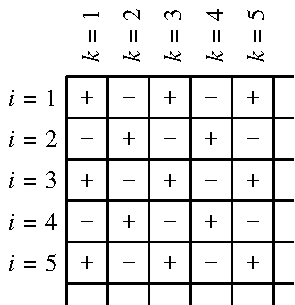
\includegraphics{2/images/schachbrett.pdf}
\end{center}

\subsubsection{Aufteilung einer Spalte}
Enthält eine Spalte nur ein einziges von Null verschiedenes Element,
können wir die Determinante auf die Berechnung einer kleineren
Determinante reduzieren.
Um dies für die Berechnung einer beliebigen Determinante ausnützen
zu können, müssen wir in der Lage sein, eine beliebige Spalte in Spalten
aufzuteilen, die nur ein einziges von Null verschiedenes Element
enthalten.
Dies gelingt mit Hilfe der Linearität.

Wir zeigen das Prinzip am Beispiel der ersten Spalte.
Die Linearität liefert
\begin{align}
\left|\begin{array}{cccc}
a_{11}&a_{12}&\dots &a_{1n}\\
a_{21}&a_{22}&\dots &a_{2n}\\
a_{31}&a_{32}&\dots &a_{3n}\\
\vdots&\ddots&\ddots&\vdots\\
a_{n1}&a_{n2}&\dots &a_{nn}\\
\end{array}\right|
&=
\left|\begin{array}{c@{\hskip2pt}c@{\hskip2pt}cccc}
a_{11}&+&  0   &a_{12}&\dots &a_{1n}\\
  0   &+&a_{21}&a_{22}&\dots &a_{2n}\\
  0   &+&a_{31}&a_{32}&\dots &a_{3n}\\
\vdots& &\vdots&\ddots&\ddots&\vdots\\
  0   &+&a_{n1}&a_{n2}&\dots &a_{nn}\\
\end{array}\right|
\notag
\\
&=
\left|\begin{array}{cccc}
a_{11}&a_{12}&\dots &a_{1n}\\
  0   &a_{22}&\dots &a_{2n}\\
  0   &a_{32}&\dots &a_{3n}\\
\vdots&\ddots&\ddots&\vdots\\
  0   &a_{n2}&\dots &a_{nn}\\
\end{array}\right|
+
\left|\begin{array}{cccc}
  0   &a_{12}&\dots &a_{1n}\\
a_{21}&a_{22}&\dots &a_{2n}\\
a_{31}&a_{32}&\dots &a_{3n}\\
\vdots&\ddots&\ddots&\vdots\\
a_{n1}&a_{n2}&\dots &a_{nn}\\
\end{array}\right|.
\label{determinate:entwicklungssatz:aufspaltung}
\end{align}
Durch wiederholte Anwendung dieser Idee kann die erste Spalte in $n$
Spalten aufgeteilt werden, die jede nur ein einziges von Null verschiedenes
Element enthält.

\subsubsection{Allgemeiner Fall}
Damit haben wir alle Komponenten für die allgemeine Berechnungsformel
zusammen.
Wir wählen dazu die Spalte $k$ aus.
Die Aufspaltungsformel
\eqref{determinate:entwicklungssatz:aufspaltung}
besagt, dass wir eine Determinante zerlegen können in eine Summe von
speziellen Determinanten, in denen die Spalte $k$ jeweils nur ein
von Null verschiedenes Elemente enthält.
Diese Elemente sind die Spaltenelemente $a_{ik}$ mit $1\le i\le n$.

Die Rekursionsformel \eqref{determinante:entwicklungssatz:rekursion}
besagt, dass wir diese Determinanten berechnen können aus der
Determinante der Matrix, in der man die Zeile $i$ und die Spalte $k$
weggelassen hat.
Die Vorzeichenregel sagt, welches Vorzeichen man dazu verwenden muss.
Insgesamt bekommen wir so die Formel
\[
\det(A)
=
\sum_{i=1}^n
\underbrace{ (-1)^{i+k}}_{\text{Vorzeichen }}
\underbrace{
a_{ik}
\cdot
\det(A_{ik}).
}_{\text{Rekursion nach 
\eqref{determinante:entwicklungssatz:rekursion}}}
\]
Sie heisst der {\em Entwicklungssatz}.
\index{Entwicklungssatz}




\subsection{Entwicklungssatz direkt aus der Linearität}
Man kann den Entwicklungssatz auch ganz direkt aus der Linearität
und den Rechenregeln für die Determinante einer Matrix $A$ herleiten.
Seien also $a_{ij}$ die Einträge in einer $n\times n$-Determinante.
Die erste Spalte können wir als Summe von Vektoren betrachten,
die jeweils nur an einer Stelle eine Eins haben und sonst aus
Nullen bestehen:
\[
\begin{pmatrix}
a_{11}\\a_{21}\\\vdots\\a_{n1}
\end{pmatrix}
=
a_{11}\begin{pmatrix}1\\0\\\vdots\\0\end{pmatrix}
+
a_{21}\begin{pmatrix}0\\1\\\vdots\\0\end{pmatrix}
+
\dots
+
a_{n1}\begin{pmatrix}0\\0\\\vdots\\1\end{pmatrix}
\]
Da die Determinante eine lineare Funktion der Spalten ist,
können wir dies einsetzen:
\begin{align*}
\det(A)
%=
%\left|\;
%\begin{matrix}
%a_{11}&a_{12}&\dots&a_{1n}\\
%a_{21}&a_{22}&\dots&a_{2n}\\
%\vdots&\vdots&\ddots&\vdots\\
%a_{n1}&a_{n2}&\dots&a_{nn}
%\end{matrix}
%\;\right|
&=
a_{11}
\left|\;
\begin{matrix}
1&a_{12}&\dots&a_{1n}\\
0&a_{22}&\dots&a_{2n}\\
\vdots&\vdots&\ddots&\vdots\\
0&a_{n2}&\dots&a_{nn}
\end{matrix}
\;\right|
+a_{21}
\left|\;
\begin{matrix}
0&a_{12}&\dots&a_{1n}\\
1&a_{22}&\dots&a_{2n}\\
\vdots&\vdots&\ddots&\vdots\\
0&a_{n2}&\dots&a_{nn}
\end{matrix}
\;\right|
+\dots
\\
&\qquad
+a_{n1}
\left|\;
\begin{matrix}
0&a_{12}&\dots&a_{1n}\\
0&a_{22}&\dots&a_{2n}\\
\vdots&\vdots&\ddots&\vdots\\
1&a_{n2}&\dots&a_{nn}
\end{matrix}
\;\right|
\end{align*}
Durch Vertauschungen kann man die Zeile, die mit $1$ beginnt, in jeder
Determinante nach oben bringen, die einzelnen Terme erhalten dadurch
alternierende Vorzeichen
\begin{align*}
\det(A)
&=
a_{11}
\left|\;
\begin{matrix}
1&a_{12}&\dots&a_{1n}\\
0&a_{22}&\dots&a_{2n}\\
\vdots&\vdots&\ddots&\vdots\\
0&a_{n2}&\dots&a_{nn}
\end{matrix}
\;\right|
-a_{21}
\left|\;
\begin{matrix}
1&a_{22}&\dots&a_{2n}\\
0&a_{12}&\dots&a_{1n}\\
\vdots&\vdots&\ddots&\vdots\\
0&a_{n2}&\dots&a_{nn}
\end{matrix}
\;\right|
+\dots
\\
&\qquad
+(-1)^{n+1}a_{n1}
\left|\;
\begin{matrix}
1&a_{n2}&\dots&a_{nn}\\
0&a_{12}&\dots&a_{1n}\\
0&a_{22}&\dots&a_{2n}\\
\vdots&\vdots&\ddots&\vdots\\
0&a_{n-1,2}&\dots&a_{n-1,n}
\end{matrix}
\;\right|
\end{align*}
Um die einzelnen Determinanten zu berechnen, muss man jetzt 
den Gauss-Algorithmus anwenden.
In der ersten Zeile und Spalte
gibt es nichts mehr zu tun, das dort stehende Pivot-Element ist
bereits $1$.
Es bleibt also nur noch die $(n-1)\times(n-1)$-Matrix
im rechten unteren Teil, diese besteht aus den Zeilen und Spalten
von $A$ die übrig bleiben, wenn man die erste Spalte wegstreicht,
und im $i$-ten Summanden die $i$-te Zeile.
Der Gauss-Algorithmus wird
die Determinante dieser $(n-1)\times(n-1)$ Matrix liefern.
\begin{align*}
\det(A)
&=
a_{11}
\left|\;
\begin{matrix}
a_{22}&\dots&a_{2n}\\
a_{32}&\dots&a_{3n}\\
\vdots&\ddots&\vdots\\
a_{n2}&\dots&a_{nn}
\end{matrix}
\;\right|
-a_{21}
\left|\;
\begin{matrix}
a_{12}&\dots&a_{1n}\\
a_{32}&\dots&a_{3n}\\
\vdots&\ddots&\vdots\\
a_{n2}&\dots&a_{nn}
\end{matrix}
\;\right|
+\dots
\\
&\qquad
+(-1)^{n+1}a_{n1}
\left|\;
\begin{matrix}
a_{12}&\dots&a_{1n}\\
a_{22}&\dots&a_{2n}\\
\vdots&\ddots&\vdots\\
a_{n-1,2}&\dots&a_{n-1,n}
\end{matrix}
\;\right|
\end{align*}
Wir verwenden folgende Notation, um diese Formel noch etwas kompakter
auszudrücken.
\index{Minor}
\begin{definition}Sei $A$ eine $n\times n$-Matrix mit Einträgen $a_{ij}$.
Dann heisst die Matrix $A_{ij}$, die sich aus $A$ durch wegstreichen
der $i$-ten Zeile und der $j$-ten Spalte ergibt, der $i$-$j$-Minor der
Matrix $A$.
\end{definition}
Damit kann der Determinantenentwicklungssatz nun wie folgt formuliert
werden:
\begin{satz}
Sei $A$ eine $n\times n$-Matrix.
Dann ist
\[
\det(A)=
\sum_{i=1}^n(-1)^{i+1}a_{i1}\det(A_{i1})
=
\sum_{i=1}^n(-1)^{1+j}a_{1j}\det(A_{1j})
\]
die Entwicklung nach der ersten Spalte bzw.~Zeile, und 
\[
\det(A)=
\sum_{i=1}^n(-1)^{i+j}a_{ij}\det(A_{ij})
=
\sum_{j=1}^n(-1)^{i+j}a_{ij}\det(A_{ij})
\]
die Entwicklung nach der $j$-ten Spalte bzw.~$i$-ten Zeile. 
\end{satz}

\begin{beispiel}Die zu Beginn des Kapitels gefundene Formel für
die Determinante einer $2\times 2$-Matrix ist ein Spezialfall
des Entwicklungssatzes
\[
\left|\;
\begin{matrix}
a&b\\c&d
\end{matrix}
\;\right|
=a\cdot\det(d)-b\cdot\det(c)=ad-bc.
\]
\end{beispiel}

\begin{beispiel}
Man berechne die Determinante der Matrix
\[
A=\begin{pmatrix}
-1&-3&0\\
2&3&-2\\
2&1&-3
\end{pmatrix}
\]
Der Entwicklungssatz liefert
\begin{align*}
\det(A)&=
-1\det\begin{pmatrix}3&-2\\1&-3\end{pmatrix}
-2\det\begin{pmatrix}-3&0\\1&-3\end{pmatrix}
+2\det\begin{pmatrix}-3&0\\3&-2\end{pmatrix}
\\
&=
-1(-9+2)-2(9-0)+2(6-0)=7-18+12=1.
\end{align*}
\end{beispiel}

\subsection{Spezialfall: Dimension 3, die Sarrus Formel}
\index{Sarrus-Formel}
Mit diesem Satz lässt sich jetzt auch die Sarrussche Formel einfach beweisen:
\begin{align*}
\left|\;
\begin{matrix}
a_{11}&a_{12}&a_{13}\\
a_{21}&a_{22}&a_{23}\\
a_{31}&a_{32}&a_{33}
\end{matrix}\;\right|
&=
a_{11}
\left|\;\begin{matrix}
a_{22}&a_{23}\\
a_{32}&a_{33}
\end{matrix}\;\right|
-
a_{21}
\left|\;\begin{matrix}
a_{12}&a_{13}\\
a_{32}&a_{33}
\end{matrix}\;\right|
+
a_{31}
\left|\;\begin{matrix}
a_{12}&a_{13}\\
a_{22}&a_{23}
\end{matrix}\;\right|
\\
&=a_{11}(a_{22}a_{33}-a_{23}a_{32})
-a_{21}(a_{12}a_{33}-a_{13}a_{32})
+a_{31}(a_{12}a_{23}-a_{13}a_{22})
\\
&=
a_{11}a_{22}a_{33}+a_{12}a_{23}a_{31}+a_{13}a_{21}a_{32}
-a_{31}a_{22}a_{13}-a_{32}a_{23}a_{11}-a_{33}a_{21}a_{12}
\end{align*}
Achtung: diese Formel kann nicht auf grössere Determinanten
verallgemeinert werden.



\subsection{Entwicklungssatz direkt aus der Linearität}
Man kann den Entwicklungssatz auch ganz direkt aus der Linearität
und den Rechenregeln für die Determinante einer Matrix $A$ herleiten.
Seien also $a_{ij}$ die Einträge in einer $n\times n$-Determinante.
Die erste Spalte können wir als Summe von Vektoren betrachten,
die jeweils nur an einer Stelle eine Eins haben und sonst aus
Nullen bestehen:
\[
\begin{pmatrix}
a_{11}\\a_{21}\\\vdots\\a_{n1}
\end{pmatrix}
=
a_{11}\begin{pmatrix}1\\0\\\vdots\\0\end{pmatrix}
+
a_{21}\begin{pmatrix}0\\1\\\vdots\\0\end{pmatrix}
+
\dots
+
a_{n1}\begin{pmatrix}0\\0\\\vdots\\1\end{pmatrix}
\]
Da die Determinante eine lineare Funktion der Spalten ist,
können wir dies einsetzen:
\begin{align*}
\det(A)
%=
%\left|\;
%\begin{matrix}
%a_{11}&a_{12}&\dots&a_{1n}\\
%a_{21}&a_{22}&\dots&a_{2n}\\
%\vdots&\vdots&\ddots&\vdots\\
%a_{n1}&a_{n2}&\dots&a_{nn}
%\end{matrix}
%\;\right|
&=
a_{11}
\left|\;
\begin{matrix}
1&a_{12}&\dots&a_{1n}\\
0&a_{22}&\dots&a_{2n}\\
\vdots&\vdots&\ddots&\vdots\\
0&a_{n2}&\dots&a_{nn}
\end{matrix}
\;\right|
+a_{21}
\left|\;
\begin{matrix}
0&a_{12}&\dots&a_{1n}\\
1&a_{22}&\dots&a_{2n}\\
\vdots&\vdots&\ddots&\vdots\\
0&a_{n2}&\dots&a_{nn}
\end{matrix}
\;\right|
+\dots
\\
&\qquad
+a_{n1}
\left|\;
\begin{matrix}
0&a_{12}&\dots&a_{1n}\\
0&a_{22}&\dots&a_{2n}\\
\vdots&\vdots&\ddots&\vdots\\
1&a_{n2}&\dots&a_{nn}
\end{matrix}
\;\right|
\end{align*}
Durch Vertauschungen kann man die Zeile, die mit $1$ beginnt, in jeder
Determinante nach oben bringen, die einzelnen Terme erhalten dadurch
alternierende Vorzeichen
\begin{align*}
\det(A)
&=
a_{11}
\left|\;
\begin{matrix}
1&a_{12}&\dots&a_{1n}\\
0&a_{22}&\dots&a_{2n}\\
\vdots&\vdots&\ddots&\vdots\\
0&a_{n2}&\dots&a_{nn}
\end{matrix}
\;\right|
-a_{21}
\left|\;
\begin{matrix}
1&a_{22}&\dots&a_{2n}\\
0&a_{12}&\dots&a_{1n}\\
\vdots&\vdots&\ddots&\vdots\\
0&a_{n2}&\dots&a_{nn}
\end{matrix}
\;\right|
+\dots
\\
&\qquad
+(-1)^{n+1}a_{n1}
\left|\;
\begin{matrix}
1&a_{n2}&\dots&a_{nn}\\
0&a_{12}&\dots&a_{1n}\\
0&a_{22}&\dots&a_{2n}\\
\vdots&\vdots&\ddots&\vdots\\
0&a_{n-1,2}&\dots&a_{n-1,n}
\end{matrix}
\;\right|
\end{align*}
Um die einzelnen Determinanten zu berechnen, muss man jetzt 
den Gauss-Algorithmus anwenden.
In der ersten Zeile und Spalte
gibt es nichts mehr zu tun, das dort stehende Pivot-Element ist
bereits $1$.
Es bleibt also nur noch die $(n-1)\times(n-1)$-Matrix
im rechten unteren Teil, diese besteht aus den Zeilen und Spalten
von $A$ die übrig bleiben, wenn man die erste Spalte wegstreicht,
und im $i$-ten Summanden die $i$-te Zeile.
Der Gauss-Algorithmus wird
die Determinante dieser $(n-1)\times(n-1)$ Matrix liefern.
\begin{align*}
\det(A)
&=
a_{11}
\left|\;
\begin{matrix}
a_{22}&\dots&a_{2n}\\
a_{32}&\dots&a_{3n}\\
\vdots&\ddots&\vdots\\
a_{n2}&\dots&a_{nn}
\end{matrix}
\;\right|
-a_{21}
\left|\;
\begin{matrix}
a_{12}&\dots&a_{1n}\\
a_{32}&\dots&a_{3n}\\
\vdots&\ddots&\vdots\\
a_{n2}&\dots&a_{nn}
\end{matrix}
\;\right|
+\dots
\\
&\qquad
+(-1)^{n+1}a_{n1}
\left|\;
\begin{matrix}
a_{12}&\dots&a_{1n}\\
a_{22}&\dots&a_{2n}\\
\vdots&\ddots&\vdots\\
a_{n-1,2}&\dots&a_{n-1,n}
\end{matrix}
\;\right|
\end{align*}
Wir verwenden folgende Notation, um diese Formel noch etwas kompakter
auszudrücken.
\index{Minor}
\begin{definition}Sei $A$ eine $n\times n$-Matrix mit Einträgen $a_{ij}$.
Dann heisst die Matrix $A_{ij}$, die sich aus $A$ durch wegstreichen
der $i$-ten Zeile und der $j$-ten Spalte ergibt, der $i$-$j$-Minor der
Matrix $A$.
\end{definition}
Damit kann der Determinantenentwicklungssatz nun wie folgt formuliert
werden:
\begin{satz}
Sei $A$ eine $n\times n$-Matrix.
Dann ist
\[
\det(A)=
\sum_{i=1}^n(-1)^{i+1}a_{i1}\det(A_{i1})
=
\sum_{i=1}^n(-1)^{1+j}a_{1j}\det(A_{1j})
\]
die Entwicklung nach der ersten Spalte bzw.~Zeile, und 
\[
\det(A)=
\sum_{i=1}^n(-1)^{i+j}a_{ij}\det(A_{ij})
=
\sum_{j=1}^n(-1)^{i+j}a_{ij}\det(A_{ij})
\]
die Entwicklung nach der $j$-ten Spalte bzw.~$i$-ten Zeile. 
\end{satz}

\begin{beispiel}Die zu Beginn des Kapitels gefundene Formel für
die Determinante einer $2\times 2$-Matrix ist ein Spezialfall
des Entwicklungssatzes
\[
\left|\;
\begin{matrix}
a&b\\c&d
\end{matrix}
\;\right|
=a\cdot\det(d)-b\cdot\det(c)=ad-bc.
\]
\end{beispiel}

\begin{beispiel}
Man berechne die Determinante der Matrix
\[
A=\begin{pmatrix}
-1&-3&0\\
2&3&-2\\
2&1&-3
\end{pmatrix}
\]
Der Entwicklungssatz liefert
\begin{align*}
\det(A)&=
-1\det\begin{pmatrix}3&-2\\1&-3\end{pmatrix}
-2\det\begin{pmatrix}-3&0\\1&-3\end{pmatrix}
+2\det\begin{pmatrix}-3&0\\3&-2\end{pmatrix}
\\
&=
-1(-9+2)-2(9-0)+2(6-0)=7-18+12=1.
\end{align*}
\end{beispiel}

\subsection{Spezialfall: Dimension 3, die Sarrus Formel}
\index{Sarrus-Formel}
Mit diesem Satz lässt sich jetzt auch die Sarrussche Formel einfach beweisen:
\begin{align*}
\left|\;
\begin{matrix}
a_{11}&a_{12}&a_{13}\\
a_{21}&a_{22}&a_{23}\\
a_{31}&a_{32}&a_{33}
\end{matrix}\;\right|
&=
a_{11}
\left|\;\begin{matrix}
a_{22}&a_{23}\\
a_{32}&a_{33}
\end{matrix}\;\right|
-
a_{21}
\left|\;\begin{matrix}
a_{12}&a_{13}\\
a_{32}&a_{33}
\end{matrix}\;\right|
+
a_{31}
\left|\;\begin{matrix}
a_{12}&a_{13}\\
a_{22}&a_{23}
\end{matrix}\;\right|
\\
&=a_{11}(a_{22}a_{33}-a_{23}a_{32})
-a_{21}(a_{12}a_{33}-a_{13}a_{32})
+a_{31}(a_{12}a_{23}-a_{13}a_{22})
\\
&=
a_{11}a_{22}a_{33}+a_{12}a_{23}a_{31}+a_{13}a_{21}a_{32}
-a_{31}a_{22}a_{13}-a_{32}a_{23}a_{11}-a_{33}a_{21}a_{12}
\end{align*}
Achtung: diese Formel kann nicht auf grössere Determinanten
verallgemeinert werden.

\section{Produktformel}
Wie verträgt sich die Determinante mit Matrizenprodukten?
Überraschenderweise gibt es hierauf eine sehr einfach Antwort,
die auch nicht schwierig zu verstehen ist.

\begin{satz}\label{detprodukt}
Sind $A$ und $B$ $n\times n$-Matrizen, dann ist
\[
\det(AB)=\det(A)\det(B).
\]
\end{satz}

\begin{proof}[Beweisidee]
Wir gehen den Beweis wie folgt an.
Wir betrachten zunächst nur die Abhängigkeit von $\det(AB)$ von $A$.
Dabei werden wir feststellen,
dass sich $\det(AB)$ fast wie die Determinante verhält, nur der
Wert für $A=E$ ist nicht der richtige, $\det(B)$ statt $1$.
Indem wir
$\det(AB)$ durch $\det(B)$ dividieren, erhalten wir aber eine Funktion,
die sich genau wie die Determinante verhält.
Weil die Eigenschaften der Determinante diese eindeutig bestimmen, muss
$\det(AB)/\det(B)=\det(A)$ sein, woraus wir die Behauptung folgern können.
\end{proof}

\begin{proof}[Beweis]
Wir betrachten die Funktion $d\colon A\mapsto d(A) = \det(AB)$.
Sie hat die folgenden Eigenschaften, die weiter unten noch
begründet werden müssen:
\begin{enumerate}
\item[1'.] $d$ ist eine lineare Funktion der Zeilen von $A$.
\item[2.']
Hat $A$ zwei gleiche Zeilen, dann auch $AB$ und damit ist $d(A)=0$.
\item[3.]
$d(E)=\det(B)$.
\end{enumerate}
Die Funktion $d$ verhält sich bis auf die letzte Eigenschaft
wie die Determinante.
Dividiert man die Funktion $d$ durch die Determinante
von $B$, ist auch die letzte Eigenschaft die einer Determinanten.
Die Funktion
\[
d':A\mapsto \frac{\det(AB)}{\det(B)}
\]
hat die Eigenschaften:
\begin{enumerate}
\item[1'.] $d'$ ist eine lineare Funktion der Zeilen von $A$.
\item[2'.] Enthält $A$ zwei gleiche Zeilen, dann ist $d'(A)=0$.
\item[3.] $d'(E)=1$.
\end{enumerate}
Nach Satz \ref{detcharacterisation} muss $d'$ die Determinante von $A$ sein:
\begin{align*}
d'(A)&=\det(A)\\
\frac{\det(AB)}{\det(B)}&=\det(A)\\
\det(AB)&=\det(A)\det(B).
\end{align*}
Das beweist die Produktformel, bis auf die oben behaupteten Eigenschaften
1' und 2'.

Die Zeile mit der Nummer $i$ in $AB$ wird erhalten,
indem man die Zeile $i$ von $A$
mit der Matrix $B$ multipliziert.
Wenn also $A$ zwei gleiche Zeilen enthält, dann sind auch die
entsprechenden Zeilen von $AB$ gleich.
was Eigenschaft 2 beweist.

Ist die Zeile $i$ von $A$ eine Linearekombination der Form
\[
\begin{pmatrix}
a_{i1}&\dots&a_{in}
\end{pmatrix}
=
\lambda
\begin{pmatrix}
a'_{i1} &\dots &a'_{in}
\end{pmatrix}
+
\mu
\begin{pmatrix}
a''_{i1} &\dots &a''_{in}
\end{pmatrix},
\]
dann ist die Zeile $i$ von $AB$ ebenfalls eine Linearekombination,
nämlich
\[
\begin{pmatrix}
a_{i1}&\dots&a_{in}
\end{pmatrix}B
=
\lambda
\begin{pmatrix}
a'_{i1} &\dots &a'_{in}
\end{pmatrix}B
+
\mu
\begin{pmatrix}
a''_{i1} &\dots &a''_{in}
\end{pmatrix}B.
\]
Schreiben wir $A'$ für die Matrix, die in Zeile $i$ die $a'_{ij}$
statt der $a_{ij}$ enthalten, und analog für $A''$, dann folgt, dass
\[
d(A) = \det(AB)=\lambda \det(A'B)+\mu\det(A''B)=\lambda d(A') + \mu d(A''),
\]
was genau die Eigenschaft 1 ist.
\end{proof}

Es gibt keine vergleichbare Formel für die Determinante der Summe
von zwei Matrizen.
Schon $2\times 2$-Diagonalmatrizen zeigen uns,
das wir eine solche Formel auch nicht erwarten können:
\begin{align*}
A&=\begin{pmatrix}a&0\\0&1\end{pmatrix}&
\det(A)&=\left|\;\begin{matrix}a  &0\\0&  1\end{matrix}\;\right|= a\\
B&=\begin{pmatrix}1&0\\0&b\end{pmatrix}&
\det(B)&=\left|\;\begin{matrix}  1&0\\0&b  \end{matrix}\;\right|= b\\
A+B&=\begin{pmatrix}a+1&0\\0&b+1\end{pmatrix}
&
\det(A+B)&=\left|\;\begin{matrix}a+1&0\\0&b+1\end{matrix}\;\right|\\
&&&=(a+1)(b+1)=ab+a+b+1.
\end{align*}
Offenbar gibt es keine einfache Formel, die $\det(A+B)$ mit $\det(A)$ und
$\det(B)$ verbindet.

\section{Lösen von Gleichungssystemen}
Aus dem Hilfssatz \ref{detlinabh} folgt sofort, dass ein Gleichungssystem
genau dann eindeutig lösbar ist, wenn die Determinante der Koeffizienten
nicht $0$ ist.

\begin{satz}
Das Gleichungssystem mit $n$ Unbekannten und $n$ Gleichungen
mit den Koeffizienten $a_{ij}$ ist genau dann eindeutig lösbar,
wenn
$\det A\ne 0$
\end{satz}

Wir möchten jetzt die in der Einleitung versprochen Formel für die Lösung
ableiten, mit der man die Lösung des Gleichungssystems aus lauter
Determinanten berechnen kann.

\index{Cramersche Regel}
\begin{satz}[Cramer]
Das Gleichungssystem mit $n$ Unbekannten und $n$ Gleichungen
mit den Koeffizienten $a_{ij}$ 
mit $\det A\ne 0$ hat die Lösungen
\[
x_1=\frac{
\left|\,\begin{matrix}
b_1&a_{12}&\dots&a_{1n}\\
\vdots&\vdots&\ddots&\vdots\\
b_n&a_{n2}&\dots&a_{nn}\\
\end{matrix}\,\right|
}{
\left|\,\begin{matrix}
a_{11}&a_{12}&\dots&a_{1n}\\
\vdots&\vdots&\ddots&\vdots\\
a_{n1}&a_{n2}&\dots&a_{nn}\\
\end{matrix}\,\right|
}
,\qquad\dots,\qquad
x_n=\frac{
\left|\,\begin{matrix}
a_{11}&\dots&a_{1,n-1}&b_1\\
\vdots&\ddots&\vdots&\vdots\\
a_{n1}&\dots&a_{n,n-1}&b_n\\
\end{matrix}\,\right|
}{
\left|\,\begin{matrix}
a_{11}&\dots&a_{1,n-1}&a_{1n}\\
\vdots&\ddots&\vdots&\vdots\\
a_{n1}&\dots&a_{n,n-1}&a_{nn}\\
\end{matrix}\,\right|
}
\]
Die Unbekannte $x_k$ berechnet man also als Quotient der Determinante
von $A$, in der man die $k$-te Spalte durch die rechten Seiten $b_i$
ersetzt hat, und der Determinanten von $A$.
\end{satz}
\begin{proof}[Beweis]
Schreiben wir $a_1,\dots,a_n$ für die Spalten von $A$ und $b$ für die 
Spalte der rechten Seite, dann bedeutet das Gleichungssystem, dass die
Spalte $b$ geschrieben werden kann als eine Linearkombination der
Spalten von $A$:
\begin{equation}
x_1a_1+\dots +x_na_n=b
\label{glinspalten}
\end{equation}
Die Determinante von $A$ ist eine lineare Funktion jeder einzelnen Spalte.
Wir betrachten für den Moment nur die Abhängigkeit von der $k$-ten
Spalte und schreiben dafür
\[
\Delta_k(u)=\left|
\,\begin{matrix}
a_{11}&\dots&u_1&\dots&a_{1n}\\
\vdots&\ddots&\vdots&\ddots&\vdots\\
a_{n1}&\dots&u_n&\dots&a_{nn}
\end{matrix}
\,\right|.
\]
Setzen wir beide Seiten von (\ref{glinspalten}) in $\Delta_k$ ein,
erhalten wir unter Ausnützung der Linearität:
\[
x_1\Delta_k(a_1)+\dots+x_k\Delta_k(a_k)+\dots+x_n\Delta_k(a_n)=\Delta_k(b).
\]
Auf der linken Seite enthalten alle Terme ausser dem $k$-ten die
Spalte $a_i$ zweimal, einmal am Platz $i$, und einmal neu eingefügt am
Platz $k$.
Da die Determinante verschwindet, wenn zwei Spalten übereinstimmen,
bleibt nur der $k$-te Term stehen:
\[
x_k\Delta_k(a_k)=\Delta_k(b)
\]
Auf der linken Seite setzt man die $k$-te Spalte als $k$-te Spalte
in $A$ ein und berechnet die Determinante, dies ist also nichts
anderes als die Determinante von $A$.
Auf der rechten Seite ersetze man die $k$-Spalte von $A$ durch $b$, also
\[
x_k
\left|\,\begin{matrix}
a_{11}&\dots&a_{1n}\\
\vdots&\ddots&\vdots\\
a_{n1}&\dots&a_{nn}\\
\end{matrix}\,\right|
=
\left|\,\begin{matrix}
a_{11}&\dots&b_1&\dots&a_{1n}\\
\vdots&\ddots&\vdots&\ddots&\vdots\\
a_{n1}&\dots&b_n&\dots&a_{nn}\\
\end{matrix}\,\right|
\]
Die Behauptung folgt jetzt durch Auflösen nach $x_k$.
\end{proof}
Dieser Satz stellt zwar eine hübsche Formel zur Berechnung der Lösung
bereit, praktisch nützlich ist diese jedoch kaum.
Die Berechnung der
$n+1$ Determinanten ist bereits aufwendiger als die Durchführung des
Gauss-Verfahrens, welches die Lösung auch schon liefert.

\begin{beispiel}Man finde die Lösung des Gleichungssystems
\[
\begin{linsys}{4}
-x&-&3y&&&=&\color[rgb]{0,0.5,0}-7\\
2x&+&3y&-&2z&=&\color[rgb]{0,0.5,0}2\\
2x&+&y&-&3z&=&\color[rgb]{0,0.5,0}-5
\end{linsys}
\]
Die Koeffizientenmatrix und die rechte Seite sind
\[
A=\begin{pmatrix}
-1&-3&0\\
2&3&-2\\
2&1&-3
\end{pmatrix}
,\qquad
b=\begin{pmatrix}
\color[rgb]{0,0.5,0}-7\\\color[rgb]{0,0.5,0}2\\\color[rgb]{0,0.5,0}-5
\end{pmatrix}
\]
wobei wir früher bereits $\det(A)=1$ gefunden haben.
Für die Lösungen des Gleichungssystems bekommen wir damit
\begin{align*}
x&=\frac{
\left|\;
\begin{matrix}
\color[rgb]{0,0.5,0}-7&-3&0\\
\color[rgb]{0,0.5,0}2&3&-2\\
\color[rgb]{0,0.5,0}-5&1&-3
\end{matrix}
\;\right|
}{\det(A)}
=63-30+0-0-14-18=1,
\\
\\
y&=\frac{
\left|\;
\begin{matrix}
-1&\color[rgb]{0,0.5,0}-7&0\\
2&\color[rgb]{0,0.5,0}2&-2\\
2&\color[rgb]{0,0.5,0}-5&-3
\end{matrix}
\;\right|
}{\det(A)}
=6+28+0-0+10-42=2,
\\
\\
z&=\frac{
\left|\;
\begin{matrix}
-1&-3&\color[rgb]{0,0.5,0}-7\\
2&3&\color[rgb]{0,0.5,0}2\\
2&1&\color[rgb]{0,0.5,0}-5
\end{matrix}
\;\right|
}{\det(A)}
=15-12-14+42+2-30=3.
\end{align*}
\end{beispiel}

\section{Inverse Matrix}
\index{inverse Matrix}
Mit den im letzten Abschnitt beschriebenen Minoren kann man jetzt auch
eine Formel für die Elemente der inversen Matrix finden.
Die inverse
Matrix von $A$ hat in ihren Spalten die Lösungen $x$ des Gleichungssystems 
$Ax=b$ für ganz spezielle rechte Seiten $b$.
Die $j$-te Spalte ist die Lösung zur rechten Seite $e_j$, dem Einheitsvektor,
der genau an der $j$-ten Stelle eine $1$ hat, und sonst aus lauter Nullen
besteht.
Nach der Cramerschen Regel kann man die $i$-te Unbekannte $x_i$
in $Ax=e_j$ mit Determinanten berechnen, nämlich
\[
x_i=(-1)^{i+j}\frac{\det(A_{ji})}{\det(A)}.
\]
Dies ist auch der Eintrag in Spalte $j$ und Zeile $i$ der inversen
Matrix $A^{-1}$:
\begin{equation}
A^{-1}
=
\frac{1}{\det(A)}
\begin{pmatrix}
\det(A_{11})&-\det(A_{21})&\det(A_{31})& \dots&(-1)^{1+n} \det(A_{n1})\\
-\det(A_{12})&\det(A_{22})&-\det(A_{32})& \dots&(-1)^{2+n} \det(A_{n2})\\
\det(A_{13})&-\det(A_{23})&\det(A_{33})& \dots&(-1)^{3+n} \det(A_{n3})\\
\vdots&\vdots&\vdots&\ddots&\vdots\\
(-1)^{n+1}\det(A_{1n})&(-1)^{n+2}\det(A_{2n})&(-1)^{n+3}\det(A_{3n})& \dots&(-1)^{n+n} \det(A_{nn})\\
\end{pmatrix}
\label{inversematrix}
\end{equation}
\begin{definition}
Die Terme in der Matrix in (\ref{inversematrix})
heissen Kofaktoren der Matrix $A$.
Sie bilden die Matrix der Kofaktoren
\begin{equation}
\operatorname{cof}(A)_{ij}=
(-1)^{i+j}\det(A_{ij})
\label{cofactor}
\end{equation}
Mit dieser Notation ist die inverse Matrix
\begin{equation}
A^{-1}=\frac1{\det(A)}\operatorname{cof}(A)^t
\label{inversecofactors}
\end{equation}
\end{definition}

Für $2\times2$-Matrizen führt dies auf die manchmal nützliche
Formel
\[
\begin{pmatrix}
a&b\\c&d
\end{pmatrix}^{-1}
=
\frac1{ad-bc}\begin{pmatrix}
d&-b\\-c&a
\end{pmatrix}
\]
Für die Berechnung der Inversen grösserer Matrizen ist die Formel
nur in ganz speziellen Fällen von Nutzen.
Die Berechnung der Inverse
mit Hilfe des Gauss-Algorithmus erfordert im allgemeinen deutlich weniger
Aufwand.
Hingegen ist die Formel für theoretische Überlegungen durchaus
interessant.
Es folgt aus ihr zum Beispiel, dass die Inverse einer
Matrix mit ganzzahligen Einträgen und Determinante $1$ wieder
lauter ganzzahlige Einträge hat.
Die Menge
\[
\operatorname{SL}_n(\mathbb Z)=\{A\in M_{n}(\mathbb Z)|\det(A)=1\},
\]
hat also die Eigenschaft, dass mit $A\in\operatorname{SL}_2(\mathbb Z)$ 
auch $A^{-1}\in\operatorname{SL}_2(\mathbb Z)$.

\begin{beispiel}
Man bestimme die Inverse der Matrix
\[
A=\begin{pmatrix}
-1&-3&1\\
2&3&-2\\
2&1&-3
\end{pmatrix}
\]
Die Determinante von $A$ kann mit der Sarrus-Formel berechnet, werden.
Sie ist
\begin{align*}
\det(A)
&=
\left|
\begin{matrix}
-1&-3& 1\\
 2& 3&-2\\
 2& 1&-3
\end{matrix}
\right|
\\
&=(-1)\cdot 3\cdot(-3) +  (-3)\cdot(-2)\cdot 2 + 1\cdot 2\cdot 1
\\&\qquad
-2\cdot 3\cdot 1-1\cdot(-2)\cdot (-1)-(-3)\cdot 2\cdot (-3)
\\
&=9+12+2 - 6-2-18=-3.
\end{align*}
Die Minoren sind
\begin{align*}
\det A_{11}&=\left|\,\begin{matrix} 3&-2\\ 1&-3\end{matrix}\,\right|
%=-9+2
=-7
&
\det A_{12}&=\left|\,\begin{matrix} 2&-2\\ 2&-3\end{matrix}\,\right|
%=-6+4
=-2
&
\det A_{13}&=\left|\,\begin{matrix} 2& 3\\ 2& 1\end{matrix}\,\right|
%=2-6
=-4\\
\det A_{21}&=\left|\,\begin{matrix}-3& 1\\ 1&-3\end{matrix}\,\right|
=8
&
\det A_{22}&=\left|\,\begin{matrix}-1& 1\\ 2&-3\end{matrix}\,\right|
=1
&
\det A_{23}&=\left|\,\begin{matrix}-1&-3\\ 2& 1\end{matrix}\,\right|
%=-1+6
=5\\
\det A_{31}&=\left|\,\begin{matrix}-3& 1\\ 3&-2\end{matrix}\,\right|
=3
&
\det A_{32}&=\left|\,\begin{matrix}-1& 1\\ 2&-2\end{matrix}\,\right|
=0
&
\det A_{33}&=\left|\,\begin{matrix}-1&-3\\ 2& 3\end{matrix}\,\right|
%=-3+6
=3
\end{align*}
Beim Hinschreiben der Inversen muss man jetzt aber beachten,
dass das Element in Zeile $i$ und Spalte $j$ der inversen Matrix
mit $A_{ji}$ gebildet wird:
\[
A^{-1}=\frac1{\det(A)}\begin{pmatrix}
+\det(A_{11})&-\det(A_{21})&+\det(A_{31})\\
-\det(A_{12})&+\det(A_{22})&-\det(A_{32})\\
+\det(A_{13})&-\det(A_{23})&+\det(A_{33})
\end{pmatrix}
=\frac1{-3}\begin{pmatrix}
-7&-8& 3\\
 2& 1& 0\\
-4&-5& 3
\end{pmatrix}
\]
Zur Kontrolle rechnen wir das Produkt nach:
\begin{align*}
\begin{pmatrix}
-7&-8& 3\\
 2& 1& 0\\
-4&-5& 3
\end{pmatrix}
\begin{pmatrix}
-1&-3& 1\\
 2& 3&-2\\
 2& 1&-3
\end{pmatrix}
&=
\begin{pmatrix}
 7-16+6&21-24+3&-7+16-9\\
-2+ 2+0&-6+ 3+0& 2- 2+0\\
 4-10+6&12-15+3&-4+10-9
\end{pmatrix}
\\
&=-3\begin{pmatrix}
1&0&0\\
0&1&0\\
0&0&1
\end{pmatrix}.
\end{align*}
Da wir in diesem Produkt die Determinanten $-3$ noch nicht berücksichtigt
haben, ist das das zu erwartende Resultat.
\end{beispiel}

\section{Eindeutigkeit der Determinante\label{deteindeutig}}
In diesem Abschnitt wollen wir zeigen, dass die Determinante
eindeutig ist.
Wir gehen dazu wie folgt vor.
Zunächst zeigen wir,
dass sich jede Determinantenberechnung auf die Berechnung der Determinanten
von sehr speziellen $A$s zurückführen lässt, nämlich solchen,
die genau eine $1$ in jeder Zeile und Spalte haben, und sonst nur
Nullen enthalten.
Im zweiten Schritt zeigen wir dann, dass diese
speziellen Determinanten in jeder Definition dasselbe geben.

Die $k$-te Spalte $a$ von $A$ kann man als lineare Kombination von
speziellen Spalten schreiben:
\[
a_k=a_{1k}
\begin{pmatrix}
1\\0\\\vdots\\0
\end{pmatrix}
+a_{2k}
\begin{pmatrix}
0\\1\\\vdots\\0
\end{pmatrix}
+\dots+
+a_{nk}
\begin{pmatrix}
0\\0\\\vdots\\1
\end{pmatrix}
\]
Setzt man dies als $k$-te Spalte in die Determinante ein (wir hatten früher
dafür die Bezeichnung $\Delta_k(a_k)$ eingeführt), kann man mit
der Linearität  die Determinante schreiben als
\[
\det A=a_{1k}\Delta_k\left(
\begin{matrix}
1\\0\\\vdots\\0
\end{matrix}
\right)
+a_{2k}
\Delta_k\left(
\begin{matrix}
0\\1\\\vdots\\0
\end{matrix}
\right)+\dots+
\Delta_k\left(
\begin{matrix}
0\\0\\\vdots\\1
\end{matrix}
\right).
\]
Die $\Delta_k$ auf der rechten Seite sind Determinanten, in denen 
eine Spalte ersetzt worden ist durch eine Spalte aus Nullen und genau
einer Eins.

Diese Zerlegung kann man jetzt noch $(n-1)$-mal wiederholen,
jedes mal kommt ein anderer Faktor $a_{ik}$ vor die Determinante.
Dabei werden auch Determinanten entsteht die die gleichen Spalten
haben, die also die Eins an der selben Stelle haben.
Diese Determinanten verschwinden alle, man kann sie ignorieren.
Der Vorfaktor ist
jeweils $a_{ik}$, wobei $i$ die Zeile der Eins bezeichnet, und $k$
die Nummer der Spalte, die man ersetzt hat.
Die Indizes des
Vorfaktors $a_{ik}$ sind gerade die Koordinaten der Eins, die durch
die Ersetzung in der Determinante stehen bleibt.

Am Ende bleibt eine Summe von Termen stehen, in der alle Determinanten
in jeder Zeile und Spalte genau eine $1$ und sonst lauter Nullen
enthalten.
Die Vorfaktoren sind die Produkte der Koeffizienten in $A$,
die an Stelle der $1$ in der ursprünglichen Matrizen standen.

Wir bezeichnen die speziellen Matrizen aus lauter Nullen und Einsen
mit $\sigma$, und die Menge all dieser Matrizen mit $S_n$.
Aus einem
Index $i$ kann man die zugehörige Spalte $k$ herausfinden, indem
man die einzige Spalte in $\sigma$ sucht, welche an der $i$-ten
Stelle eine $1$ enthält.
Wir schreiben $\sigma(i)$ für dieses $k$.
Mit dieser Schreibweise ist 
\[
\det A=\sum_{\sigma\in S_n}
a_{1\sigma(1)}
a_{2\sigma(2)}
\dots
a_{n\sigma(n)}
\det \sigma.
\]
Aus dieser Formel ist jetzt klar, dass die Determinante nicht vom
Vorgehen abhängt.

Dieselben Auflösungen kann man auch mit Hilfe der Linearität der
Determinante als Funktion der Spalten vornehmen, dabei kommt die 
gleiche Formel heraus.
Wenn man jetzt noch zeigen kann, dass
die Determinanten $\det\sigma$ nicht davon abhängen, ob man von
Zeilen oder von Spalten ausgeht, dann ist klar, dass es nur eine
Determinante gibt.

Die Determinante von $\sigma$ muss $1$ oder $-1$ sein, denn durch
Zeilenvertauschungen kann sie auf die Form $E$ gebracht werden.
Alternativ kann dies mit Spaltenvertauschungen geschehen.
Jede Vertauschung trägt einen Faktor $-1$ zum Wert der Determinante bei.
Es kommt also nur darauf an, ob die Zahl der nötigen
Vertauschungen gerade oder ungerade ist.
